% Experiments: MNIST with hand-drawn templates. Owner: claude (sentiment/MNIST thread).
\subsection{MNIST with weights that are drawings}
\label{sec:mnist}

\paragraph{Task.} MNIST digits, 10{,}000 test images. A trained linear classifier
reaches $\sim$92\%, a small MLP $\sim$97\%, a CNN $>$99\%.

\paragraph{Architecture.} Image $\to$ fixed $5\times5$ Gaussian blur $\to$ zero-mean,
unit-norm $\to$ $\mathrm{Conv2d}(1\to36,\ 28\times28,\ \mathrm{padding}\ 3)$ $\to$
max-pool over the $7\times7$ offsets ($\pm3$\,px translation tolerance) $\to$ maxout
$36\to10$ (best-matching style of each digit) $\to$ class bias $\to$ argmax. Each of
the 36 kernels is a $14\times14$ ASCII drawing typed by the author (Figure~\ref{fig:templates}),
expanded by a parameter-free function: upsample $\times2$, widen the stroke to
$\sim$3\,px with a cross kernel, blur, subtract the mean (so ink \emph{outside} the
stroke counts against the match), normalise (so the activation is a cosine). Two to
five styles were drawn per digit (a straight and a slanted 1, a 7 with and without a
bar, an open and a closed 4, a 2 with a flat and with a looped base). We count the
typed \texttt{\#} characters as the non-zero parameters: 544 blind, 662 final.

\begin{figure}[t]\centering
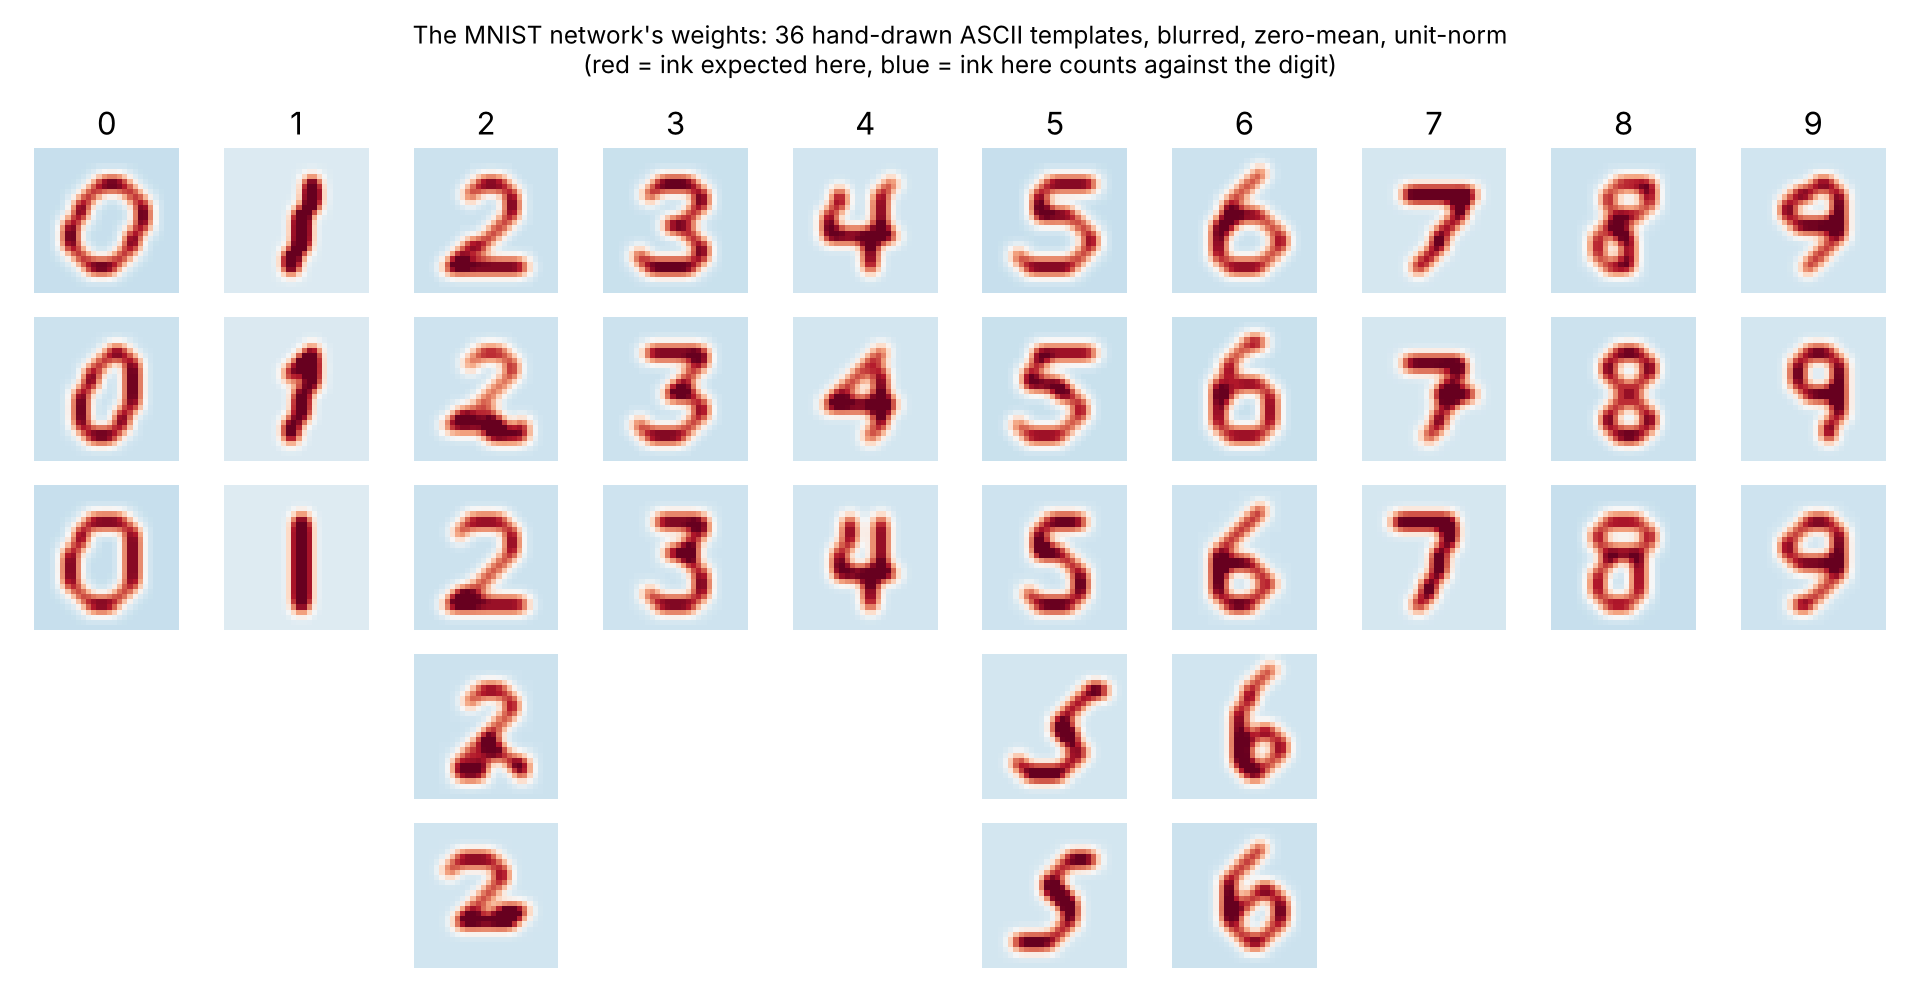
\includegraphics[width=\linewidth]{figures/mnist_templates.png}
\caption{The MNIST network's weights: 36 hand-drawn templates after expansion to
$28\times28$ kernels. Red: ink expected; blue: ink here is evidence against the digit.}
\label{fig:templates}
\end{figure}

\begin{table}[h]\centering
\begin{tabular}{lrrr}\toprule
Weights & Labels seen & Ink pixels / templates & Test acc.\\\midrule
\textbf{Hand-drawn} & 0 & 544 / 28 & \textbf{55.4\%}\\
\textbf{Hand-drawn, revision 1} & 500 (class means viewed) & 553 / 30 & \textbf{74.3\%}\\
\textbf{Hand-drawn, revision 2} & 500 (error images viewed) & 662 / 36 & \textbf{79.4\%}\\
Trained logistic regression & 50 & -- & 61.4\%\\
Trained logistic regression & 100 & -- & 71.5\%\\
Trained MLP (64 hidden) & 100 & -- & 71.8\%\\
Trained logistic regression & 500 & -- & 85.0\%\\
Trained MLP (64 hidden) & 500 & -- & 86.2\%\\
Trained logistic regression & 10{,}000 & -- & 90.9\%\\
Trained MLP (64 hidden) & 10{,}000 & -- & 95.4\%\\
\bottomrule\end{tabular}
\caption{MNIST test accuracy. The best hand-drawn network is worth about 200
labelled images.}
\label{tab:mnist}
\end{table}

\paragraph{Revisions.} The blind drawings were systematically wrong: one grid row
too high, upright rather than right-leaning, too wide. Revision~1 redrew all ten
digits after viewing the class-mean image of 500 labelled training digits next to
the templates ($+19$ points). Revision~2 added two styles each for 2, 5 and 6 (the
weakest classes) after viewing six misclassified training examples of each, widened
the blur from $3\times3$ to $5\times5$ and the shift from $\pm2$ to $\pm3$\,px
($+5$ points).

\paragraph{Why this one loses.} The large confusions are $3\to5$ (197), $4\to9$
(158), $9\to4$ (129) and $5\to8$ (106): pairs that differ in the presence of one
small stroke, which a whole-digit correlation barely registers against the shared
bulk of the shape. A trained linear classifier puts large weight on exactly those few
discriminative pixels; a person drawing a prototype cannot know which pixels those
are without seeing thousands of examples. The features that matter on MNIST are not
nameable, so the design step has nothing to work with. A part-based variant
(hand-drawn stroke detectors feeding a hand-written $10\times64$ linear layer) was
tried and abandoned: writing those 640 numbers was, on inspection, guessing.

\begin{figure}[t]\centering
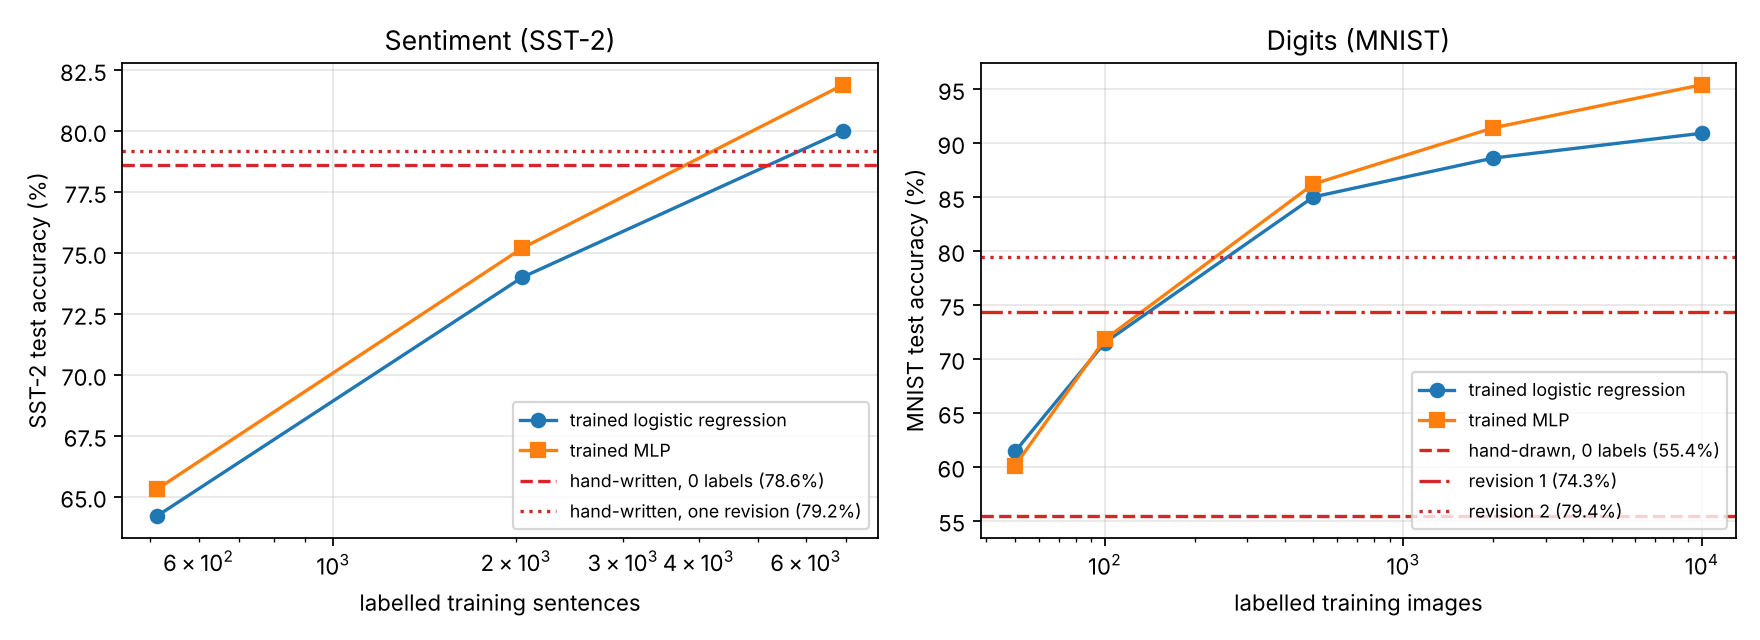
\includegraphics[width=\linewidth]{figures/label_efficiency.png}
\caption{Designed versus trained, per label. Dashed lines: hand-written networks;
curves: the same architectures trained on $2^k$ labels. Sentiment (left) and MNIST
(right) sit at the two ends of the ``nameable features'' axis.}
\label{fig:labels}
\end{figure}
